\hypertarget{anatomie-van-de-hand}{%
\section{Anatomie van de hand}\label{anatomie-van-de-hand}}

Handen zijn uiterst belangrijk voor de mens, omdat mensen met de hand in
staat hun omgeving te manipuleren en ook essentiële levensbehoeften
vervullen, zoals eten en drinken. Handen zijn erg kenmerkend voor de
mens. De menselijke hand wijkt erg af van wat vele dieren hebben.

De menselijke hand wordt gekenmerkt door opponeerbare duimen, wat
betekent dat mensen met het topje van hun duim hun andere vingers aan
kunnen raken. Bij veel dieren is dit niet het geval.

\begin{figure}
\centering
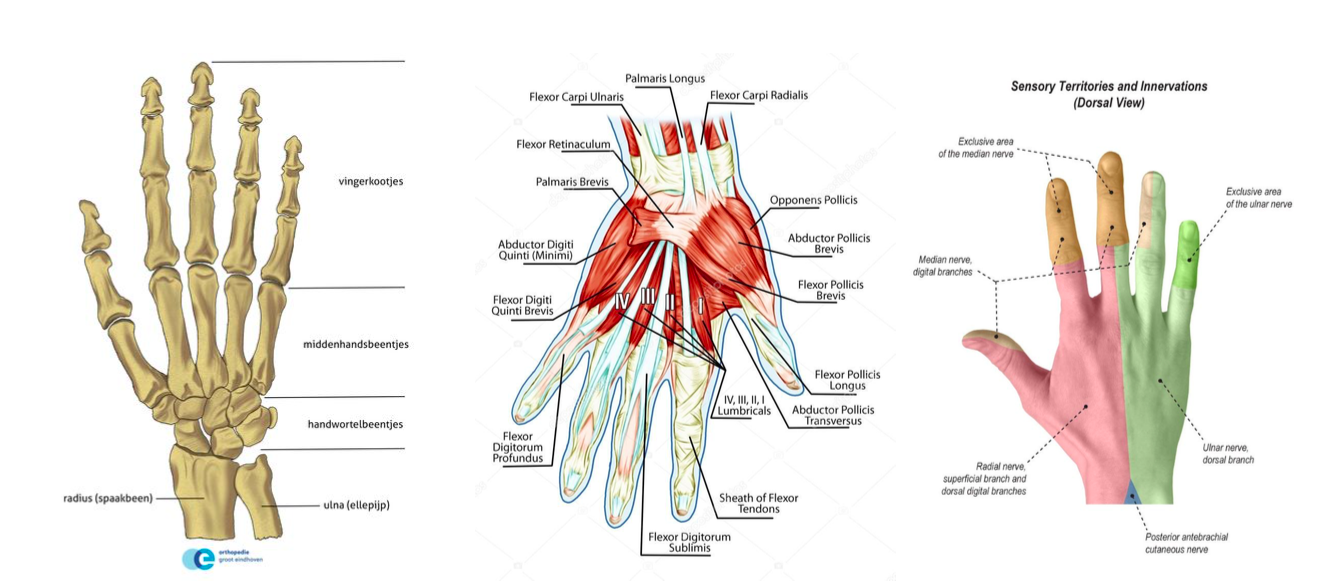
\includegraphics[width=1\textwidth,height=\textheight]{img/anatomie.png}
\caption{Anatomie van de hand. V.l.n.r: Beenderen, spieren en pezen en
zenuwen\label{fig:anatomie}}
\end{figure}

\hypertarget{beenderen}{%
\subsection{Beenderen}\label{beenderen}}

De hand bestaat wel uit 27 kleine botjes (``Natuurinformatie - Hand''
z.d.). De botjes zorgen ervoor dat de handen, en met name de vingers
ervan, erg beweegbaar zijn. De duim kan wel 90 graden worden gedraaid,
in tegenstelling tot de andere vingers. Deze kunnen ongeveer 45 graden
worden gedraaid.

De onderarm eindigt met de ellepijp en het spaakbeen. Hier gaat het over
naar de pols, deze bestaat uit acht handwortelbeentjes. Hier zijn alle
vingers aan bevestigd. Boven de handwortelbeentjes, in de middenhand,
bevinden zich de middenhandsbeentjes. Dit maakt de pols beweegbaar,
zodat het makkelijker is om voorwerpen vast te grijpen. De vingers
bestaan uit vingerkootjes. Bij elke vinger zijn dit er drie, behalve de
duim, deze heeft er twee. Hierdoor is een vinger in drie delen te
krommen. In de geneeskunde en anatomie worden deze vingers vaak
aangeduid met romeinse cijfers. Dit loopt van digitus I (de duim) tot
digitus V (de pink), zoals ook gebruikt in Alpenfels (1955).

\hypertarget{spieren-en-pezen}{%
\subsection{Spieren en pezen}\label{spieren-en-pezen}}

De spieren in de hand worden verdeeld onder twee soorten: de intrinsieke
en extrinsieke banden. Intrinsieke banden zijn kort en stijf en bevinden
zich vooral in de handpalm. Deze spieren hoeven namelijk niet sterk uit
te rekken. Extrinsieke banden zijn soepeler en een stuk langer. Zij
verbinden de onderarmbotten met de middenhandsbeentjes, Mortelé (2009).
Wanneer deze worden aangespannen, buigen de vingers.

Ook bevindt het CMC-gewricht, Oosterbos en Koot (z.d.), zich in de hand.
Dit gewricht maakt het mogelijk de duim in oppositie te bewegen, dit
betekent dat de duim naar de pink wordt bewogen. Hierdoor kan men de
duim in veel meer verschillende posities houden dan de andere vier
vingers. Dit maakt de menselijke hand ook zo complex.

In de hand bevinden zich ook pezen die het te ver terugbuigen van de
vingers voorkomen. Als deze er niet waren, zouden de vingers makkelijk
de verkeerde kant op buigen, hetgeen zorgt voor het scheuren van andere
spieren.

\hypertarget{zenuwen-en-aderen}{%
\subsection{Zenuwen en aderen}\label{zenuwen-en-aderen}}

De hand is voorzien van drie gemengde zenuwen: de nervus ulnaris, nervus
medianus en nervus radialis. Deze zenuwen sturen de spieren in de hand
en onderarm aan. De zenuwen hebben alle drie zowel motorische
(`bewegende') als sensibele (`voelende') functie. Deze sensibele functie
laat een hoge haptische waarneming toe, wat betekent dat je erg veel kan
voelen met de hand. Bijvoorbeeld druk-, bewegings- en
vibratiestimulansen. De bloedtoevoer wordt verzorgd door twee slagaders:
de arteria radialis en arteria ulnaris.

\hypertarget{gouden-ratio-in-de-anatomie-van-de-hand}{%
\subsection{Gouden ratio in de anatomie van de
hand}\label{gouden-ratio-in-de-anatomie-van-de-hand}}

De gouden ratio of gulden snede is een speciale wiskundige verdeling van
een lijnstuk. De gouden ratio is al vanaf de oudheid bestudeerd. Dit
omdat het vaak in de natuur voor blijkt te komen. De gouden ratio op
lijnstuk AB (\xrefname{Fig.}\cref{fig:lijn}) met punt S als de gouden
ratio is te definiëren als:

\[ \phi_{1} = \frac{1+\sqrt{5}}{2} \approx 1,618\dots \] (``Gulden
snede'' z.d.)

Dit ratio blijkt massaal voor te komen in de natuur. De gouden ratio
wordt door velen gezien als de meest esthetische verhouding in zowel
kunst, natuur en design, benoemd in Osborne (1999). In de natuur kan men
denken aan de groente romanesco en verschillende bloemblaadjes.

\begin{figure}
\centering
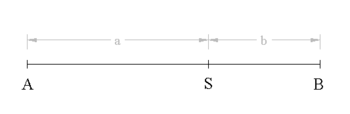
\includegraphics[width=0.36\textwidth,height=\textheight]{img/image_7.png}
\caption{Lijnstuk AB met punt S als gouden ratio\label{fig:lijn}}
\end{figure}

Maar ook in de anatomie blijkt de gulden snede voor te komen.
Bijvoorbeeld in de arm. Zie \xrefname{Fig.}\cref{fig:goudenanatomie}.
Onze vingers bestaan uit 3 delen. De eerste twee delen (blauwe B en C in
figuur 7). Zijn in gouden ratio met de totale lengte van de vinger. Ook
staan de middelvinger en pink in deze verhouding met elkaar. Murali
(2012).

\begin{figure}
\centering
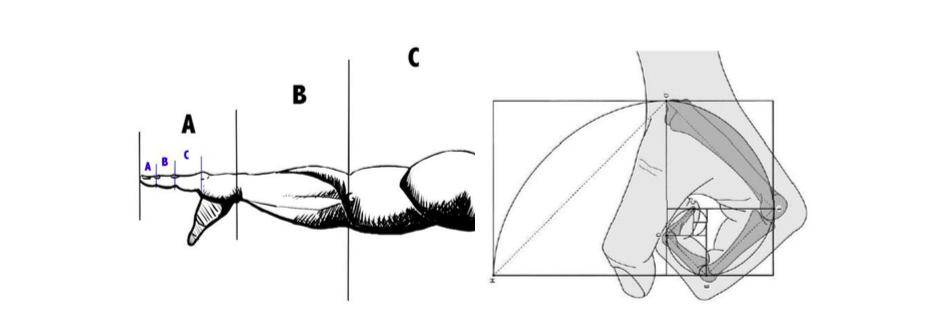
\includegraphics[width=1\textwidth,height=\textheight]{img/goudenanatomie.png}
\caption{Gouden ratio in de anatomie\label{fig:goudenanatomie}}
\end{figure}

De rij van Fibonacci houdt sterk verband met de gulden snede. Deze
interessante reeks begint met 0 en 1, waarbij elk volgend element de som
van beiden elementen hiervoor is. Dit geeft voor de eerste tien getallen
de volgende reeks:

\(0, 1, 1, 2, 3, 5, 8, 13, 21, 34 \dots\) (``Rij van Fibonacci'' z.d.)

Als men dit vervolgens plot op een (oneindig) rechte lijn, is het gouden
ratio duidelijk te visualiseren. Ook nadert de reeks het gouden ratio
als zijnde een limiet.
